	En este capítulo comparamos los resultados de la ejecución de 5 modelos, los tiempos de ejecución de cada modelo en PowerDEVS comparándolos con 
	el modelo transformado en QSS-Solver. 
	Los modelos ejecutados, tanto los originales en PowerDEVS como los modelos transformados en $\mu$-Modelilca se encuentran en 
	\url{https://github.com/lucciano/pd2mo/tree/master/doc/tesina/src}

\section{Comparación de desempeño}
	A continuación por cada uno de los modelos se muestra su modelo en PowerDEVS seguido de dos gráficas (ambas son generadas con GNUPlot). 
	A la izquierda se muestra el resultado de la simulación de PowerDEVS y a la derecha el resultado del modelo transformado en el QSS-Solver.

	Las simulaciones fueron llevadas acabo en una PC Intel\textsuperscript{\textregistered} Core\textsuperscript{TM} i7-3632QM CPU @ 2.20GHz con 16 GB de memoria RAM. Los tiempos observados no deben ser considerados como absolutos ya que variarán de un sistema a otro, aunque las mejoras relativas se mantendrán.


\section{Ecuaciones Lotka-Volterra}

	El sistema de ecuaciones Lotka-Volterra fue presentado en la página \pageref{lotka_volterra_ref}, el cual es un sistema de ecuaciones diferenciales de primer orden, no lineales, utilizadas para describir dinámicas de sistemas biológicos en el cual dos especies interactúan, una como presa y otra como depredador y se definen como:

\begin{align*}
\frac{dx}{dt} & = x(\alpha - \beta y)\\
\frac{dy}{dt} & =y(\gamma - \delta  x)
\end{align*}

donde:
\begin{itemize}
	\item y es el número de algún predador (por ejemplo, un lobo);
    \item x es el número de sus presas (por ejemplo, conejos);
    \item t representa el tiempo; y
    \item $\alpha$, $\beta$, $\gamma$, $\delta$ son parámetros que representan las interacciones de las dos especies.
\end{itemize}

	Este sistema es representado en PowerDEVS por el modelo de la Figura \ref{model:lotka_volterra}:

\begin{figure}[H]
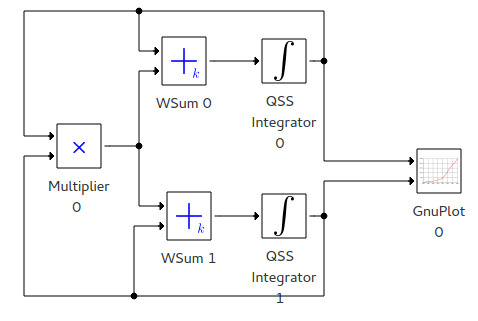
\includegraphics[width=0.75\linewidth]{lotka_voltera_pwd}
\caption{Modelo PowerDEVS del Sistema Lotka Volterra}
\label{model:lotka_volterra}
\end{figure}

\begin{figure}[H]
\centering
\begin{minipage}{0.5\textwidth}
\centering
 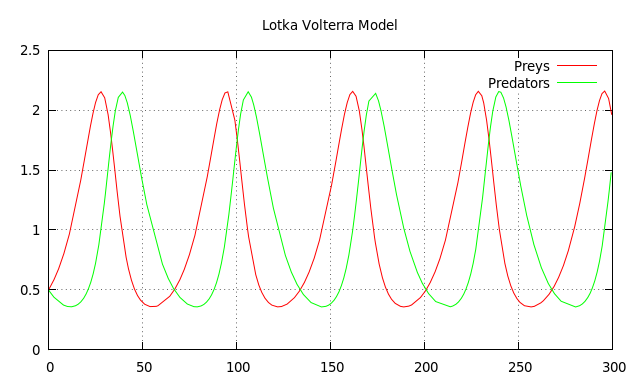
\includegraphics[width=\linewidth]{lotka_voltera-pd}
PowerDEVS \\
\end{minipage}\hfill
\begin{minipage}{0.5\textwidth}
\centering
 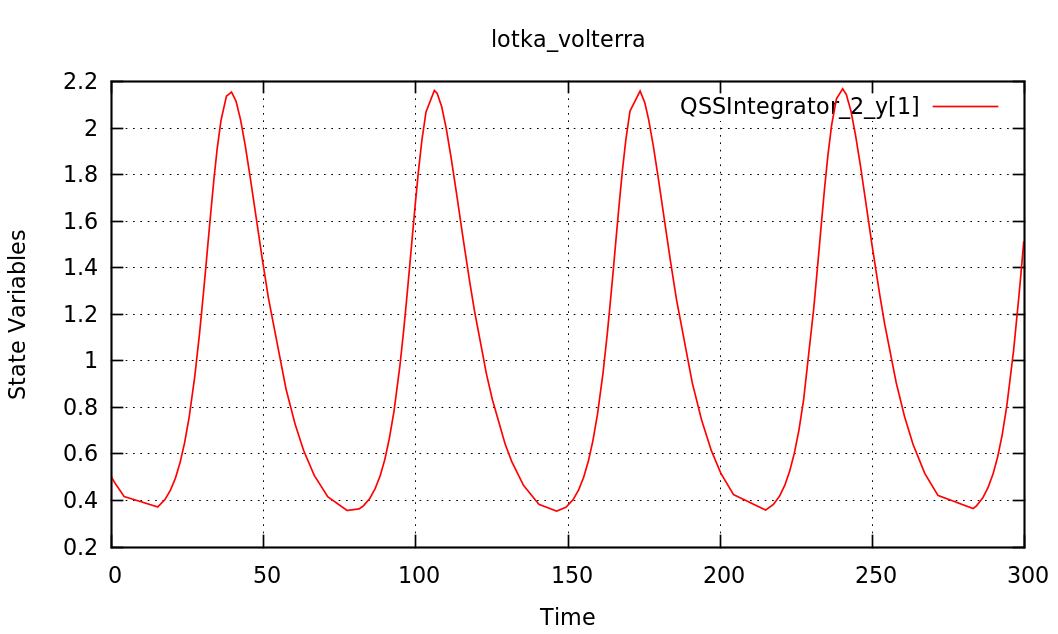
\includegraphics[width=\linewidth]{lotka_voltera-qss}
QSS-Solver \\
\end{minipage}
\label{graph:lotka_voltera}
\caption{Resultados de la simulación del Modelo Lotka Volterra}
\end{figure}

En la Figura \ref{graph:lotka_voltera} se pueden ver los dos resultados de la simulación de 300 segundos. A la izquierda el resultado en PowerDEVS, el cual tomó 11 ms,
y a la derecha el resultado en QSS-Solver el cual tomó 2.75 ms.

\section{Líneas de Transmisión}
	El siguiente sistema de ecuaciones representa un modelo de una línea de transmisión formada por $N$ secciones de circuitos LC:

\begin{equation}
\begin{split}
\frac{d v_{j}}{d t} &= \frac{i_{j} - i_{j+1}}{C} \\
\frac{d i_{j}}{d t} &= \frac{v_{j-1} - v_{j}}{L} \\	
\end{split}
\end{equation}

para $j = 2 \dots N$

Consideramos un pulso de entrada:
\begin{equation}
v_0(t) = \left\{ 
  \begin{array}{l l}
    1 \text{ si } t < 1 \\
    0 \text{ en caso contrario }
  \end{array} \right.
\end{equation}

En la Figura \ref{model:lclines} se puede ver el modelo de PowerDEVS para la simulación del modelo de Líneas de Transmisión.

\begin{figure}[H]
 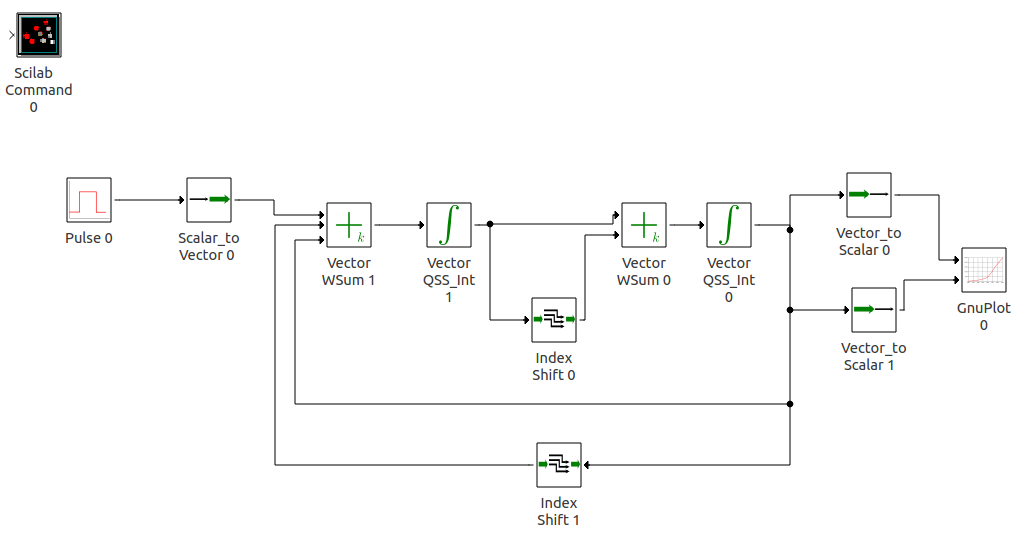
\includegraphics[width=0.75\linewidth]{lclines}
\label{model:lclines}
\caption{Modelo PowerDEVS de Líneas de Transmisión}
\end{figure}

\begin{figure}[H]
\centering
\begin{minipage}{0.5\textwidth}
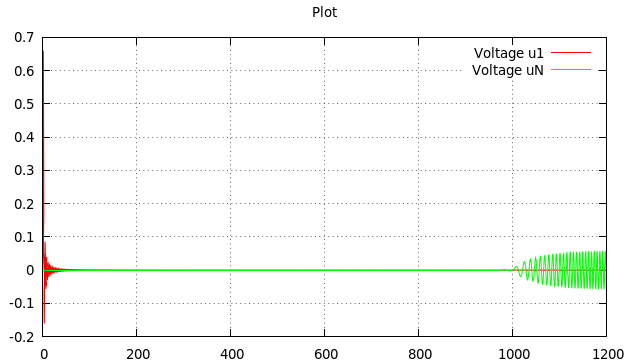
\includegraphics[width=\linewidth]{lcline-pd}
PowerDEVS\\
\end{minipage}\hfill
\begin{minipage}{0.5\textwidth}
 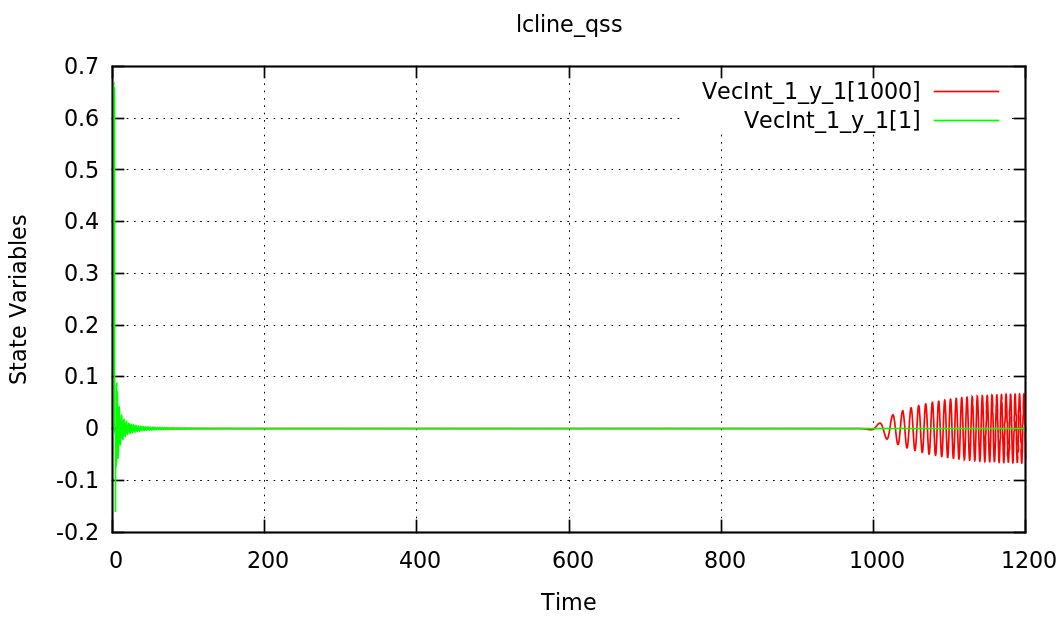
\includegraphics[width=\linewidth]{lcline-qss}
QSS-Solver\\
\end{minipage}
\caption{Resultados de la simulación de Líneas de Transmisión}
\label{graph:lclines}
\end{figure}

En la Figura \ref{graph:lclines} se puede ver el resultado de la simulación de 20 minutos (1200 s) del Modelo de Líneas de Transmisión con 1000 segmentos en PowerDEVS,
	la cual tomó 76402 ms a la izquierda, mientras que a la derecha se encuentra el resultado del modelo convertido ejecutado en QSS-Solver con los mismos 
	parámetros, el cual tomó 34982.5 ms.

\section{Inversores Lógicos}
	El siguiente modelo representa una cadena de $m$ inversores lógicos, 

\begin{align*}
\frac{d \omega_1}{d t} & = U_{op} - \omega_1(t) - \Upsilon g (u_{in}(t), \omega_{1} (t))    \\
\frac{d \omega_j}{d t} & = U_{op} - \omega_j(t) - \Upsilon g (\omega_{j-1}(t), \omega_{j} (t)) \textrm{ donde $j = 2, 3, .., m$}
\end{align*}

donde :
\begin{equation*}
	g(u, v) = (max(u - U_{thres} , 0))^2 - (max (u - v - U_{thres} , 0))^2
\end{equation*}

Se utillizaron los parametros: $\Upsilon = 100$,  $U_{thres} = 1$, y $U_{op} = 5$.
Las condiciones iniciales son : $w_j = 6.247 \cdot 10^{-3}$ para valores inpares de j y $w_j = 5$ para valores pares de $j$
La entrada es una señal periodica trapezoidal, con parametros 
$V_{up} = 5V$ , $V_{low} = 0V$, $T_{down} = 10$, $T_{up} = 5$, $T_{rise} = 5$, y $T_{fall} = 2$.
El cual es representado por el modelo PowerDEVS de la Figura \ref{model:inverters}.

\begin{figure}[H]
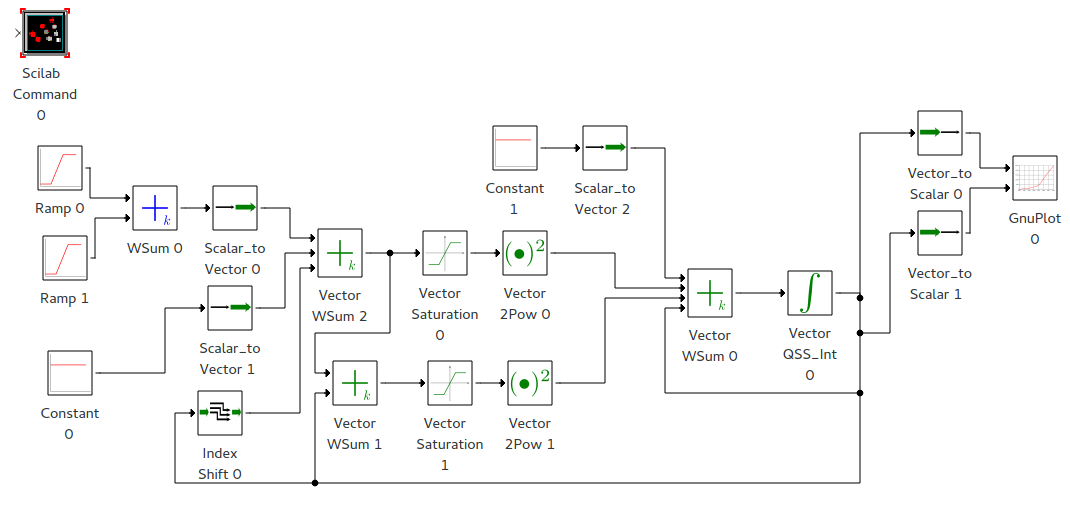
\includegraphics[width=0.75\linewidth]{inverters}
\caption{Modelo PowerDEVS de Inversores Lógicos}\label{model:inverters}
\end{figure}

\begin{figure}[H]
\centering
\begin{minipage}{0.5\textwidth}
 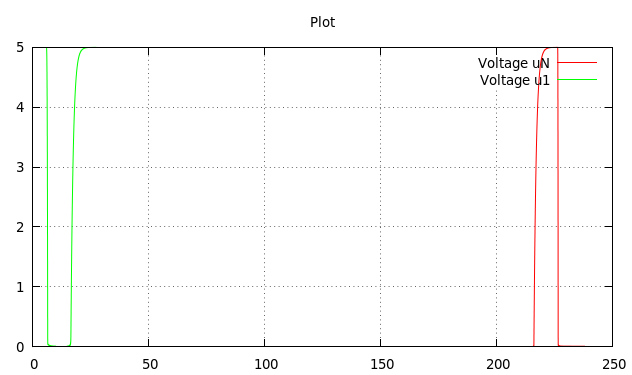
\includegraphics[width=\linewidth]{inversers-pd}
\centering
PowerDEVS
\end{minipage}\hfill
\begin{minipage}{0.5\textwidth}
 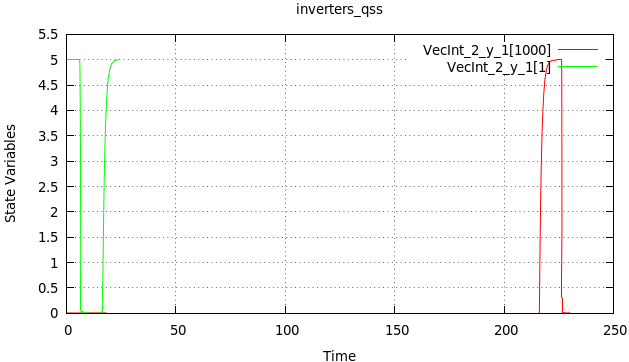
\includegraphics[width=\linewidth]{inversers-qss}
\centering
QSS-Solver
\end{minipage}
\caption{Resultados de la simulación de Inversores}\label{graph:inverters}
\end{figure}

En la Figura \ref{graph:inverters} se puede ver el resultado de la simulación del modelo de 1000 inversores durante 250 segundos, lo cual tomó 25046 ms en PowerDEVS en 
	la izquierda, mientras que en QSS-Solver tomó 7694.44 ms	

\section{Advection-Diffusion-Reaction}
	El modelo de ecuaciones Advection-diffusion-reaction (ADR) provee las bases para describir fenómenos de transferencias de calor y masa, donde la cantidad de interés $u(x,t)$ puede ser temperatura en la conducción de calor o concentración de una sustancia química.

La ecuación 
\begin{equation*}
\frac{du(x,t)}{dt} + a \frac{du(x,t)}{dx} = d\frac{d^2u(x,t)}{d^2x} + r(u(x,t)^2 - u(x,t)^3)
\end{equation*}
corresponde al modelo ADR, donde $a$,$d$ y $r$ son parámetros expresando coeficientes de advección, difusión y reacción, 
el cual es aproximado mediante el método de las lineas \cite{BKP13} en el modelo de la Figura \ref{model:adr}

\begin{figure}[H]
 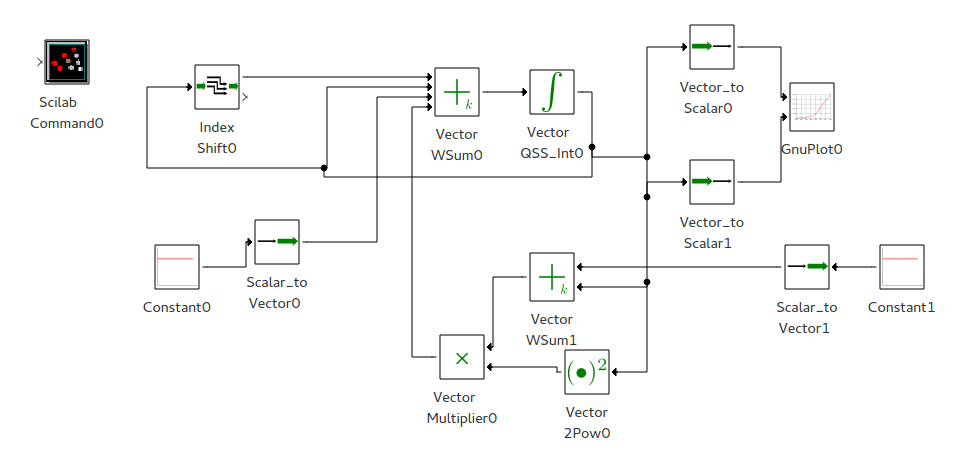
\includegraphics[width=0.75\linewidth]{adr-pwd}
\caption{Modelo PowerDEVS ADR}\label{model:adr}
\end{figure}

\begin{figure}[H]
\begin{minipage}{0.5\textwidth}
 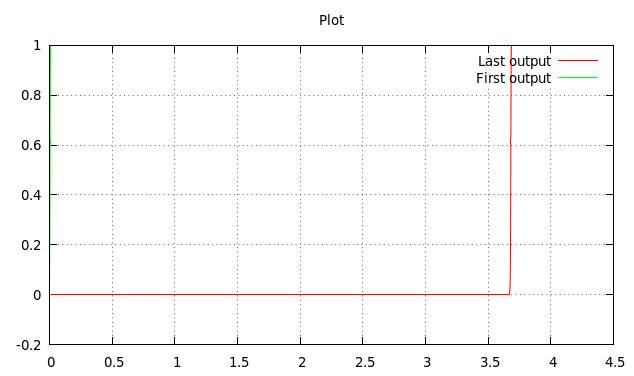
\includegraphics[width=\linewidth]{adr-pd}
\centering
PowerDEVS
\end{minipage}\hfill
\begin{minipage}{0.5\textwidth}
 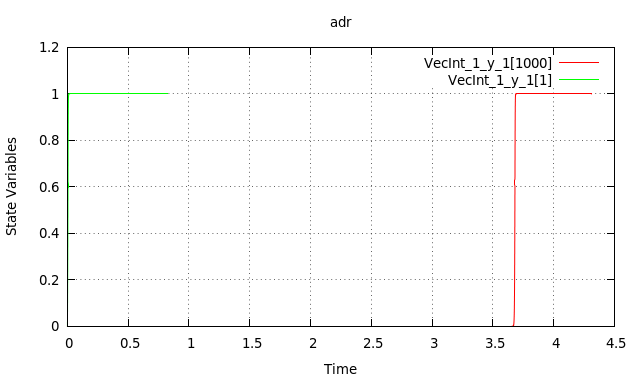
\includegraphics[width=\linewidth]{adr-qss}
\centering
QSS-Solver
\end{minipage}
\caption{Resultados de la simulación ADR}\label{graph:adr}
\end{figure}

En la Figura \ref{graph:adr} se puede ver el resultado de la simulación del modelo ADR de 10s para $N=1000$ en PowerDEVS a la izquierda, la cual tomó 6089 ms,
mientras que la simulación QSS-Solver del modelo convertido es 568.772 ms, en ambos casos utilizando el método de integración LIQSS2.

\section{Convertidor de Voltaje}
	El siguiente modelo es un tipo de convertidor DC - DC que obtiene a su  salida  un  voltaje  continuo  menor  que  a  su entrada, manteniendo una una  alta eficiencia (superior al 95\% con circuitos integrados) y autorregulación.

\begin{align*}
\frac{di_{L}}{dt} & = \frac{-u_{C} - R_D i_D }{L}\\
\frac{du_C}{dt} & =i_D \frac{i_D}{C} - \frac{u_C}{R_L C }
\end{align*}
donde
\begin{align*}
i_D & = \frac{R_s i_L - u_C - U }{R_D + R_s}
\end{align*}

Las ecuaciones anteriores se ven reflejadas en el circuito eléctrico de la Figura \ref{buckdisk-squema}.

\begin{figure}[H]
\centering
 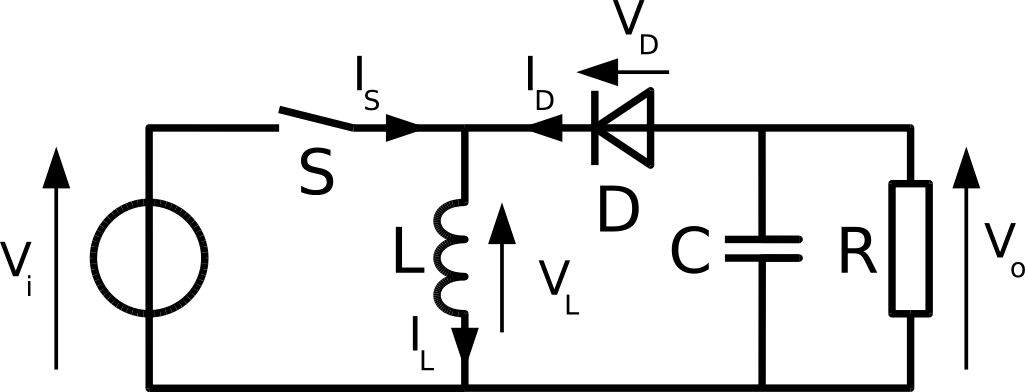
\includegraphics[width=.60\linewidth]{Buckboost_conventions}
 \caption{Esquema eléctrico de convertidor de voltaje}\label{buckdisk-squema}
\end{figure}


\begin{figure}[H]
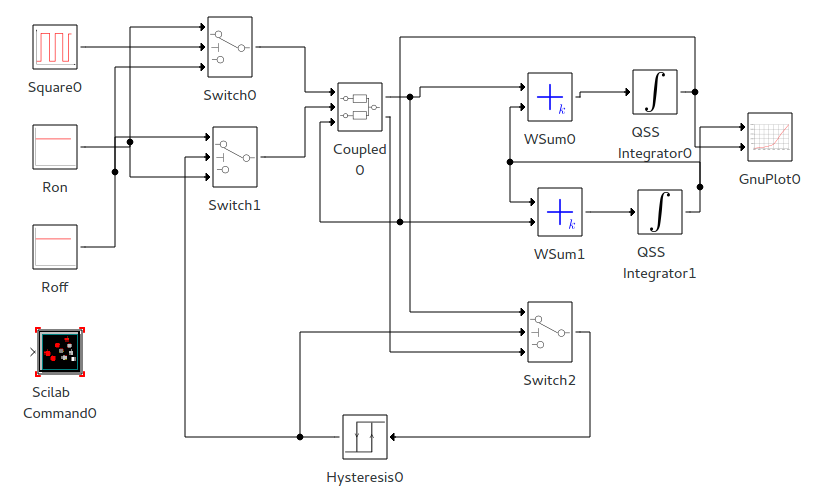
\includegraphics[width=0.75\linewidth]{buck_disk}
\caption{Modelo Convertidor de voltaje}\label{model:buckdisk}
\end{figure}

\begin{figure}[H]
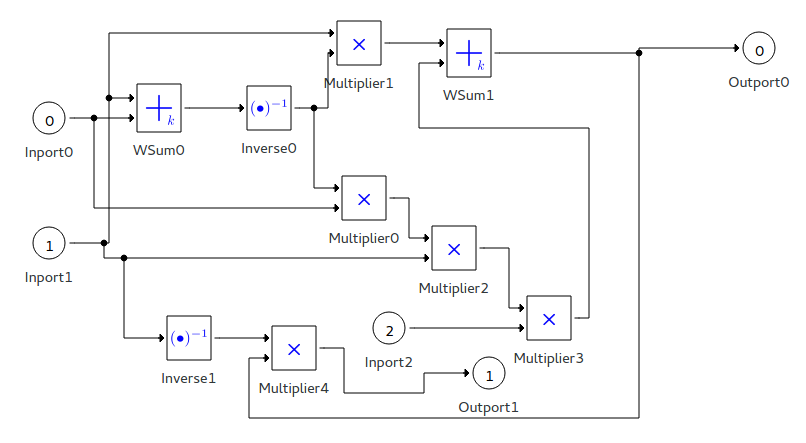
\includegraphics[width=0.75\linewidth]{buck_disk_coupled0}
\caption{Coupled0 (Incluido en Convertidor de voltaje)}\label{model:buckdiskcoupled0}
\end{figure}

El cual es representado en el modelo de la Figuras \ref{model:buckdisk} y \ref{model:buckdiskcoupled0}.

\begin{figure}[H]
\begin{minipage}{0.5\textwidth}
 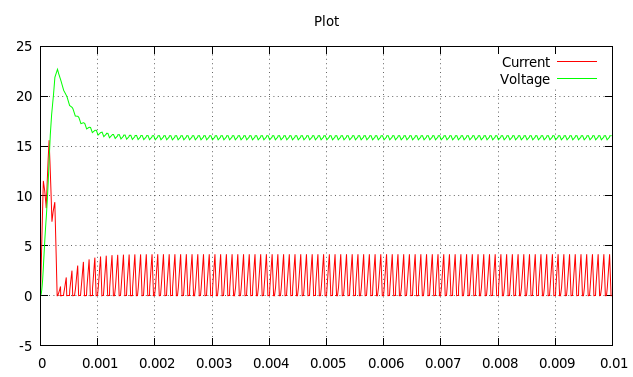
\includegraphics[width=\linewidth]{buck_disk-pd}
\centering
PowerDEVS
\end{minipage}\hfill
\begin{minipage}{0.5\textwidth}
 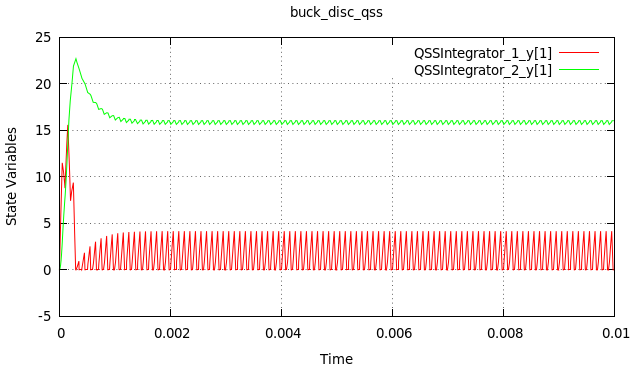
\includegraphics[width=\linewidth]{buck_disk-qss}
\centering
QSS-Solver
\end{minipage}
\caption{Resultados de la simulación de Convertidor de voltaje}
\label{result:buckdisk}
\end{figure}

En la Figura \ref{result:buckdisk} se puede ver el resultado del modelo de Convertidor de voltaje durante 0.01 s a la izquierda en PowerDEVS, lo cual tomó 268 ms, 
mientras que a la derecha se encuentra el resultado obtenido del QSS-Solver, el cual tomó 10 ms.

\section{Resultados}

	En el cuadro \ref{tab:result} se muestran los tiempos de ejecución obtenidos de los 5 modelos descriptos en este capítulo en  
	PowerDEVS (P.DEVS) y QSS-Solver (QSS-S). Ambas mediciones son reportadas por los motores de simulación, en milisegundos (ms).
	Todas las simulaciones utilizan el método de integración QSS3 excepto los que se especifica LIQSS2.

\begin{table}[H]
\centering	
\begin{tabular}{llllll}
\toprule
{\bf Modelos}            &  {\bf P.DEVS(ms)} & {\bf QSS-S. (ms)} & {\bf Mejora (\%)} \\
\toprule
Lotka  Voltera 300 s      		& 11            & 2.75132         & 81 \\
Lineas de Transmisión 1200 s, N=1000     & 76402         & 34982.5         & 54          \\
Inversores(LIQSS2) 250 s, N=1000   	& 25046         & 7694.44         & 69        \\
ADR(LIQSS2) 10 s, N=1000 		& 6089          & 568.772         & 90        \\
Convertidor de Voltaje 0.01 s,        	& 268           & 10.3802         & 96         

% Mejora esta calculada a partir de 1 - qsssolver / pwdevs
%excepto indicado, se utiliza QSS3
\end{tabular}
\caption{Comparación de las diferentes simulaciones y sus mejoras}\label{tab:result}
\end{table}

	En el cuadro \ref{tab:result} se puede ver una mejora entre 54 y 96\% entre todos los modelos.
	Los modelos vectoriales, son nuestro principal objetivo, ya que es una forma simple de describir grandes modelos y son susceptible a tener grandes mejoras
	en los tiempos de ejecución. Entre estos modelos se aprecia una mejora entre entre 54 y 90\%.
